\documentclass[../HAFiscal]{subfiles}
\begin{document}
	
\FloatBarrier
\section{Comparing fiscal stimulus policies}
\label{sec:comparing}

In this section we present our results where we compare three policies to provide fiscal stimulus in our calibrated model. The policies we compare are a means tested stimulus check, an extension of unemployment benefits, and a payroll tax cut. Each policy is implemented at the start of a recession, and we compare results both with and without aggregate demand effects being active during the recession. First, we present impulse responses of aggregate income and consumption after the implementation of each policy. Then we compare the policies in terms of their cummulative multipliers and in terms of their effect on a welfare measure that we introduce. Finally, based on these comparisons, we can rank the three policies. 

\subsection{Impulse responses}
\label{sec:IRFs}

The impulse responses that we present for each stimulus policy are constructed as follows: 
\begin{itemize} 
	\item A recession hits in quarter $1$. 
	\item We compute the subsequent path for the economy without any policy introduced in response to the recession. 
	\item We also compute the subsequent path for the economy with a given policy introduced at the onset of the recession in quarter 1. 
	\item The impulse responses we present are then the \textit{difference} between these two paths for the economy and show the effect of a policy relative to a case where no policy was implemented.
	\item The solid lines show these impulse responses for an economy where the aggregate demand effects described in section~\ref{sec:ADeffects} are not active, and the dashed lines show impulse repsonses for an economy where the aggregate demand effects are active during the recession. 
	\item Red lines refer to aggregate labor and transfer income, and blue lines refer to consumption. 
\end{itemize}

Note that all graphs show the response of income and consumption for an average recession. Specifically, we simulate recessions lasting from only one quarter up to 20 quarters. We then take the sum of the results across all recessions lengths weighted by the probability of this recession length occuring (given our assumption of an average recession length of six quaters).

\subsubsection{Stimulus check} 

\begin{figure}
	\centering
	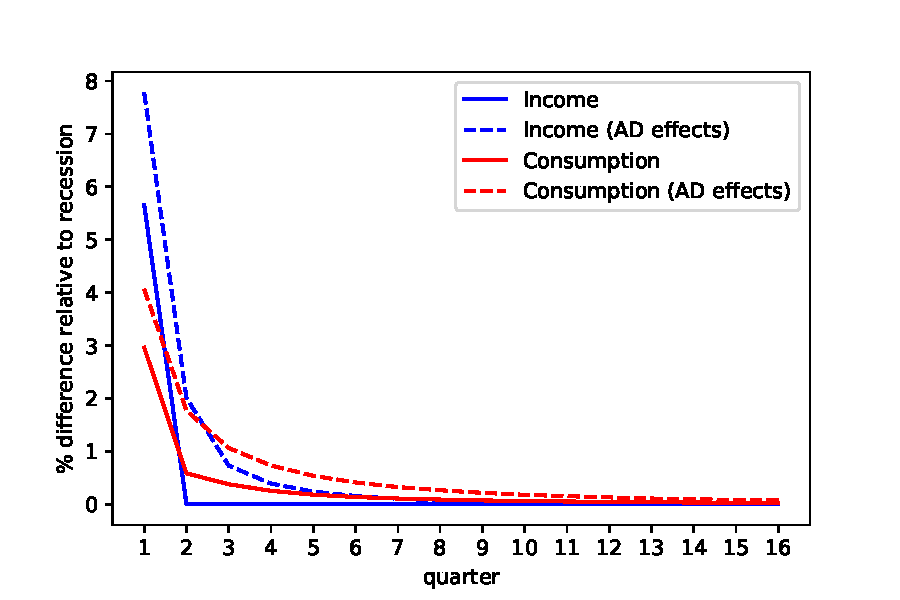
\includegraphics[width=0.8\linewidth]{Code/HA-Models/FromPandemicCode/Figures/recession_Check_relrecession}
	\caption{Impulse responses of aggregate income and consumption to a \textbf{stimulus check} during recesssions with and without aggregate demand effects}
	\label{fig:recessioncheckrelrecession}
\end{figure}

Figure \ref{fig:recessioncheckrelrecession} shows the impulse response of income and consumption when stimulus checks are issued in the first quarter of a recession. In the model without a multiplier, the stimulus checks account for over 5 percent of the first quarter's income. In the following quarters there are no further stimulus payments and income remains the same as it would have done without the stimulus check policy. Consumption is about 3 percent higher in the first quarter which includes the splurge response to the stimulus check. Consumption then drops to well below one percent above the counterfactual and the remainder of the stimulus check money is then spent over the next few years. In the model with aggregate demand effects, income in the first quarter is almost 8 percent higher than the counterfactual as the extra spending feeds into higher incomes. Consumption in this model jumps to a higher level than without aggregate demand effects and comes down more slowly as the feedback effects from consumption to income dampen the speed with which income---and hence the splurge---return to zero. After a couple of years, when the recession is most likely over and aggregate demand effects are no longer in place, income is close to where it would be without the stimulus check policy although consumption remains somewhat elevated.

\subsubsection{UI extension}

\begin{figure}
	\centering
	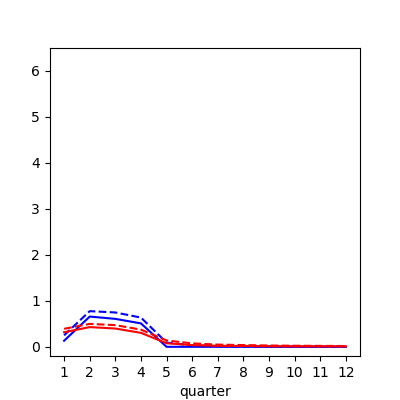
\includegraphics[width=0.8\linewidth]{Code/HA-Models/FromPandemicCode/Figures/recession_UI_relrecession}
	\caption{Impulse responses of aggregate income and consumption to a \textbf{UI extension} during recesssions with and without aggregate demand effects}
	\label{fig:recessionuirelrecession}
\end{figure}

The impulse responses in figure \ref{fig:recessionuirelrecession} show the response to a policy that extends unemployment benefits from 6 months to 12 months for a period of a year. The path for income, in the model without aggregate demand effects, now depends on the number of consumers who receive the extended unemployment benefits. These consumers are those who have been unemployed for between 6 and 12 months. In the first quarter of the recession the newly unemployed receive unemployment benefits regardless of whether they are extended or not. Therefore, it is in the second and third quarter, when the effects of the recession on long-term unemployment start to materialize, that the extended unemployment insurance payments ramp up. By the fifth quarter, the policy is no longer in effect and income from extended unemployment goes to zero. Consumption in the first quarter jumps up by more than income, prompted both by the increase in expected income and also the reduced need for precautionary saving given the extended insurance. In the model without aggregate demand effects, consumption is only a little above the counterfactual by the time the policy is over. In the model with aggregate demand effects, there is an extra boost to income of about the same size in the first and second quarters. As this extra aggregate-demand induced income goes to employed consumers, more of it is saved and consumption remains elevated several quarters beyond the end of the policy.

\subsubsection{Payroll tax cut}

\begin{figure}
	\centering
	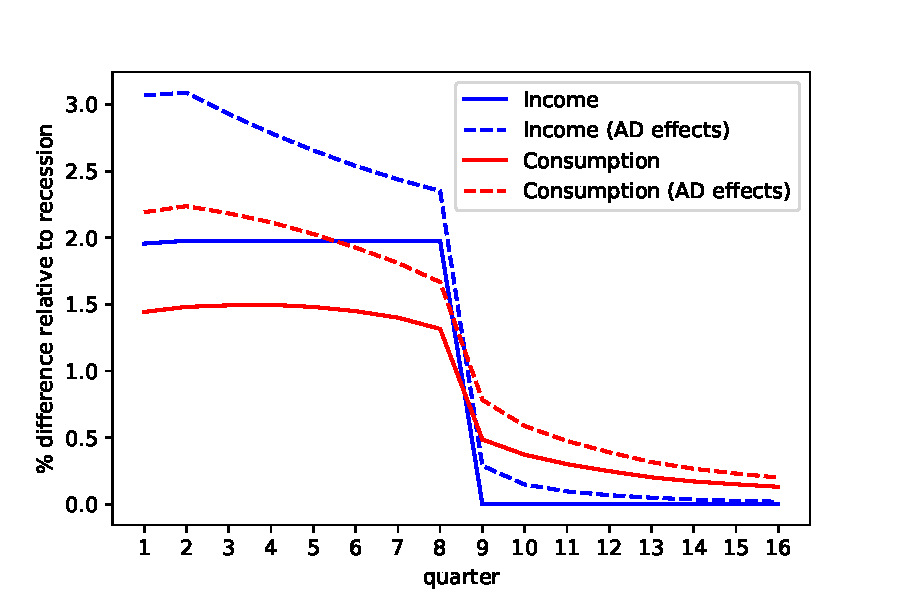
\includegraphics[width=0.8\linewidth]{Code/HA-Models/FromPandemicCode/Figures/recession_taxcut_relrecession}
	\caption{Impulse responses of aggregate income and consumption to a \textbf{payroll tax cut} lasting eight quarters during recesssions with and without aggregate demand effects}
	\label{fig:recessiontaxcutrelrecession}
\end{figure}

The final impulse response graph, Figure \ref{fig:recessiontaxcutrelrecession}, shows the impulse response for a payroll tax cut that persists for two years (8 quarters). In the model without aggregate demand effects, income rises by two percent as the take-home pay for employed consumers goes up. After the two year period, income drops back to where it would have been without the payroll tax cut. Consumption jumps close to 1.5 percent in response to the tax cut. Over the period in which the tax cut is in effect, consumption rises somewhat as the stock of precautionary savings goes up, before declining in anticipation of the drop in income at the two year mark. Following the drop in income, consumption drops due to the splurge and then decreases over time as consumers spend out the savings they built up over the period the tax cut was in effect. In the model with aggregate demand effects, income rises over three percent above the counterfactual and then declines steadily as the probability that the recession remains active, and hence the aggregate demands effects in place, goes down over time.\footnote{Again, consumption tends to first rise due to the build-up of precautionary savings, before falling again as the probability that the recession remains in place declines. This hump-shaped pattern feeds through to income, explaining the upward trend in income during the first two quarters.} In response to the now declining expected path for income over the two years during which the tax cut remains in place, consumption also declines, albeit at a slightly slower pace. Following the end of the policy, the savings stock in the model with aggregate demand effects is high and consumption remains significantly elevated through the period shown.

\subsection{Multipliers}
\label{sec:multipliers}

In this section we compare the fiscal multipliers across the three stimulus policies. Specifically, we employ the cumulative multiplier, which captures the ratio between the net present value (NPV) of stimulated consumption up to horizon $t$ and the full-horizon NPV of the cost of the policy. We thus define the cumulative multiplier up to horizon $t$ as:
\begin{equation*}
	M(t) = \frac{NPV(t,\Delta C)}{NPV (\infty,\Delta G)},
\end{equation*}
where $\Delta C$ is the additional aggregate consumption spending up to time $t$ in the policy scenario relative to the baseline and $\Delta G$ is the total government expenditure caused by the policy. The net present value of a variable $X_t$ is given by 
$NPV(t,X) = \sum_{s=0}^{t} \left( \prod_{i=1}^{s} \frac{1}{R_i} \right) X_s$. 

\begin{figure}[t]
	\centering
	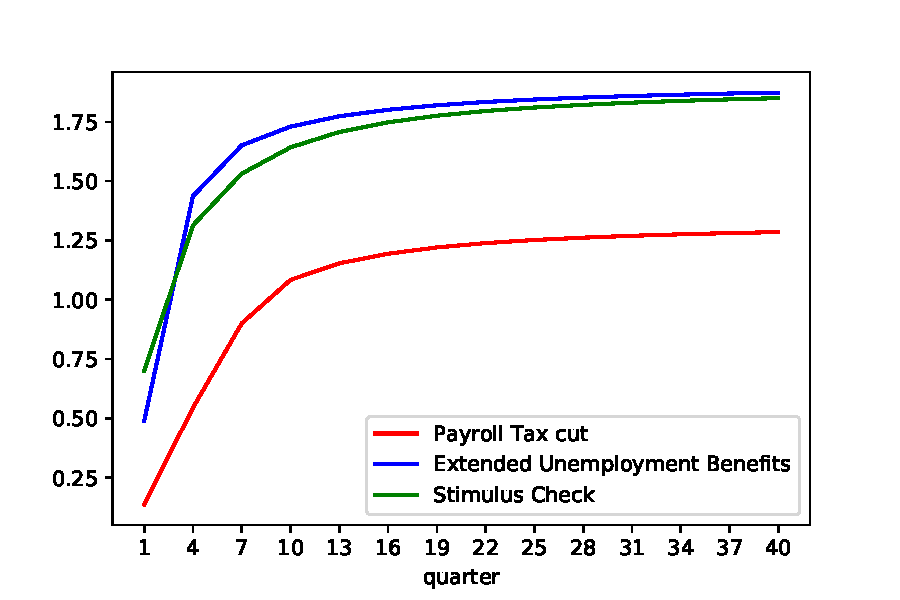
\includegraphics[width=0.8\linewidth]{Code/HA-Models/FromPandemicCode/Figures/Cummulative_multipliers}
	\caption{Cummulative Multiplier as a function of the horizon for the three policies. Policies are implemented during a recession with AD effect active.}
	\label{fig:cumulativemultipliers}
\end{figure}

Figure \ref{fig:cumulativemultipliers} plots the cumulative multipliers at different horizons, and Table~\ref{tab:Multiplier} shows the long-run multiplier for each policy. The stimulus check, which is paid out in quarter one, exhibits the largest multiplier on impact. About 70 percent of the total policy expenditure is immediately spent by consumers. After one year and due to the aggregate demand effects, consumption has increased cumulatively by more than the cost of the stimulus check. Over time, the policy reaches a total multiplier of 1.85.

The multiplier is very similar for the UI extension policy. However, since policy spending here is spread out over four quarters (and peaks in quarter two to three), the multiplier in the first quarter is considerably lower than in the case of the stimulus check. The UI extension policy is very targeted in the sense that it provides additional income to only those consumers, who due to unemployment, have large MPCs. However, some of the spending occurs at later quarters, when the recession might have ended. Overall, around 80 percent of the policy expenditure occurs during the recession. In contrast, the stimulus check is paid out fully during the first quarter when, by construction, the recession occurs with certainty. Therefore, the aggregate demand effects are particularly potent for this policy. Hence, while being less targeted and providing stimulus also to agents with low MPCs, the stimulus check ends up with a relatively high overall multiplier due to concentration of spending during the recession.

\begin{table}[t]
	\center
	\input Code/HA-Models/FromPandemicCode/Tables/Multiplier.tex
	\caption{Long-run cumulative multipliers as well as the share of the policy ocurring during the recession}
	\label{tab:Multiplier}
\end{table}

The payroll tax cut has the lowest multiplier irrespective of the considered horizon. A multiplier of 1 is reached only after around 8 quarters. The total multiplier over the whole simulated period is at approximately 1.3. These relatively small numbers reflect that policy spending lasts for a long time and is thus more likely to occur after the recession has ended. Moreover, only employed consumers with often relatively low MPCs benefit directly from the payroll tax cut. Therefore, the policy is poorly targeted if the goal is to provide short-term stimulus. 

Table \ref{tab:Multiplier} contains an additional (middle) row that shows the long-run multiplier for a special case. The aggregate demand effect works through several rounds. First, consumers increase spending due to the stimulus by the policy, which increases income, which in turn boosts consumption. However, this boost in consumption triggers another round of aggregate demand effects, with each round being subsequently smaller in magnitude. The middle row of the table shows the multipliers that result in the special case where we only consider the first-round AD effect. In the case of the tax cut, approximately half of the total stimulus effect occurs in the first round, with that value being somewhat larger for the other two policies. This reflects that the stimulus impact of the tax cut hinges to a larger extent on spillovers from the direct beneficiaries of the policy to those indirectly affected by the aggregate demand effect than is the case for the stimulus check or the UI extension, which directly target high MPC households.


\subsection{Welfare}
\label{sec:welfare}

In this section we look at the welfare implications of each stimulus policy. To do so we need a way to aggregate welfare in our model with individual utility functions. Our approach to constructing a welfare measure is based on three ideas:
\begin{enumerate}
	\item The utility of each consumer is valued equally by the social planner.
	\item There is no social benefit to implementing any of the policies outside of a recession. 
	\item Utility is gained from `splurge' spending in the same way as other spending.
\end{enumerate} 

The first of these would suggest a simple aggregation of individual wel...

Let  $\mathcal{W}(\text{policy},Rec,AD)$ be the aggregated utility function:
\begin{align}
	\mathcal{W}(\text{policy},Rec,AD) =\frac{1}{N}\sum_{i=1}^{N} \sum_{t=0}^{\infty} \beta_S^t u(c_{it,\text{policy},Rec,AD}) 
\end{align}
where $\text{policy}\in \{\text{None, Stimulus Check, UI extension, Payroll Tax Cut}\}$ is the stimulus policy followed, $Rec\in\{1,0\}$ is an indicator for whether the policy coincides with the start of a recession or is implemented in non-recessionary times, and $AD\in\{1,0\}$ is and indicator for whether the aggregate demand effects are active during the recession or not. $c_{it,\text{policy},Rec,AD}$ are the consumption paths (including the splurge) for each consumer $i$ in each scenario. $\beta_S$ is the social planner's discount factor that we will set to be equal to the inverse of the real interest rate $R$. $N$ is the number of consumers simulated.

We use the steady-state baseline as a way to convert from welfare units to consumption units. Using this baseline, we define the marginal increase in welfare that occurs when every consumer increases their consumption proportionally to their baseline consumption as:\footnote{Note that with log utility, $\mathcal{W}^c =\frac{1}{N}\sum_{i=1}^{N} \sum_{t=0}^{\infty} \beta_S^t = \frac{1}{1-\beta_S}$}
\begin{align}
	\mathcal{W}^c =\frac{1}{N}\sum_{i=1}^{N} \sum_{t=0}^{\infty} \beta_S^t c_{it,\text{None},0,0} u'(c_{it,\text{None},0,0}) .
\end{align}
With this definition we consider, in steady-state consumption units $\mathcal{W}^c$, the increase in welfare induced by a policy: $\frac{\mathcal{W}(\text{policy},Rec,AD)-\mathcal{W}(\text{None},Rec,AD)}{\mathcal{W}^c}$. The present value of the fiscal payments made by the government for each policy is $PV(\text{policy},Rec)$.\footnote{For the stimulus check and extended unemployment insurance the payments made by the government are clearly defined and do not depend on aggregate demand effects. For the payroll tax cut, we define the payments as the difference between the take-home pay with and without the tax cut, but ignoring any aggregate demand effects. Aggregate demand effects would increase the value of the tax cut, because incomes would rise, but in fact increase rather than decrease the tax receipts of the government.} We subtract the fiscal cost of each policy in steady-state consumption units:  $\frac{PV(\text{policy},Rec)}{{P}^c}$ where ${P}^c$, the marginal cost of increasing every consumer's steady-state consumption proportionally, is given by:
\begin{align}
	\mathcal{P}^c = \frac{1}{N}\sum_{i=1}^{N} \sum_{t=0}^{\infty} R^{-t} c_{it,\text{None},0,0} .
\end{align}
Finally, we normalize the welfare benefit by subtracting the welfare effect of the policy in non-recessionary times. This can be thought to encompass both the preferences of society not to redistribute and the negative incentive effects of redistribution in normal times. Our final welfare measure, expressed in units of steady-state consumption, is:
\begin{align}
	\mathcal{C}(\text{policy},Rec,AD) &= \bigg(\frac{\mathcal{W}(\text{policy},Rec,AD)-\mathcal{W}(\text{None},Rec,AD)}{\mathcal{W}^c} - \frac{PV(\text{policy},Rec)}{\mathcal{P}^c} \bigg)\\ \nonumber
	& \qquad -
	\bigg(\frac{\mathcal{W}(\text{policy},0,0) - \mathcal{W}(\text{None},0,0)}{\mathcal{W}^c} - \frac{PV(\text{policy},0)}{\mathcal{P}^c} \bigg) \label{welfare_defn}
\end{align}

Table \ref{welfare} shows the welfare benefits of each policy as defined by equation \eqref{welfare_defn}. The stimulus check and payroll tax cut policies have been adjusted to be the same fiscal size as the unemployment insurance extension.\footnote{As shown in appendix \ref{app:CheckMultiplier}, the multiplier of the check stimulus is insensitive to its size. Hence, the downscaling of the stimulus check does not alter the impact on consumption per unit of policy expenditure.} Without aggregate demand effects (the first row of the table), the payroll tax cut has extremely limited welfare benefits. This is because the payroll tax cut goes to consumers who remain employed and therefore does not directly affect the unemployed consumers who are the most hit by the recession. However, employed consumers do reduce their consumption at the onset of the recession due to the increased unemployment risk, so the tax cut helps them more than in non-recessionary times.  Similarly, the stimulus check has limited benefit as it mostly goes to employed consumers although it has the benefit over the payroll tax cut of also reaching the unemployed. The extended unemployment insurance policy is the clear `bang for the buck' winner as all the payments go to unemployed households who are likely to have significantly higher marginal utility for consumption than in non-recessionary times.

The second row of the table shows the welfare benefits in the version of the model with aggregate demand effects during the recession. The payroll tax cut now has a noticeable benefit as some of the tax cut gets spent during the recession resulting in higher incomes for all consumers. However, the tax cut is received over a period of two years, and much of this may be after the recession---and hence the aggregate demand effect---is over. Furthermore, because the payroll tax cut goes only to employed consumers who have relatively lower MPCs, the spending out of this stimulus will be further delayed possibly beyond the period of the recession. By contrast, the stimulus check is received in the first period of the recession and goes to both employed and unemployed consumers. The earlier arrival and higher MPCs of the stimulus check recipients means more of the stimulus is spent during the recession leading to greater aggregate demand effects, higher income, and higher welfare. The extended unemployment insurance arrives, on average, slightly later than the stimulus check. However, the recipients, who have been unemployed for at least six months, spend the extra benefits relatively quickly resulting in significant aggregate demand effects during the recession. In contrast to the payroll tax cut, extended unemployment insurance has the benefit of automatically reducing if the recession ends early and less consumers are eligible for the benefit.

\begin{table}[ht] 
	\center
	\input Code/HA-Models/FromPandemicCode/Tables/welfare4.tex
	\caption{Consumption equivalent welfare gains in basis points, calculated for policies implemented in a recession with and without aggregate demand effects}
	\label{welfare}
\end{table}

\subsection{Comparing the policies} 

The results presented in section~\ref{sec:multipliers} and~\ref{sec:welfare} indicate that the extension of unemployment benefits is the clear `bang for the buck' winner. 
(TODO: discuss targeting vs timing of spending)





\end{document}	